\textbf{\underline{\large{3.3: Context For Definite Integrals: Area, Displacement, and Net Change}}} \par

Since we originally defined the definite integral in terms of ``area under a curve,'' we need to consider what this idea of ``area'' really means in relation to the definite integral. \par

Recall \textbf{Ex 3.2.2}, where we had a function $y = x\cos \left(x^2\right)$ on $x \in \left[0 \, \sqrt{\pi}\right]$. The graph looks like this: \\

\begin{center}
    \includegraphics[width = 0.6\textwidth]{\graphicsdir Chapter 3 Graphics/3.3-Graphic1.png}
\end{center}

In \textbf{Ex 3.2.2}, we found that $\int_0^{\sqrt{\pi}} x\cos \left(x^2\right) \, dx = 0 \forcespace$. But, there's clearly area under the curve, so how can the integral equal both the area and 0? Well, as it turns out, because the integral was created from rectangles with width $dx$ and height $f(x)$, a negative $f(x)$ will result in a rectangle with ``negative area.'' Take a look at the following graph: \\

\begin{center}
    \includegraphics[width = 0.6\textwidth]{\graphicsdir Chapter 3 Graphics/3.3-Graphic2.png}
\end{center}

It's clear that by our definition of the definite integral, the ``area'' in red would cancel out the ``area'' in blue. So, how would we find the actual, positive area? That is what we are going to talk about in this section. \par

\begin{tcolorbox}[objective]
    \begin{center}
        OBJECTIVES \\[11pt]
    \end{center}
    Relate Definite Integrals to Area Under a Curve. \\
    Understand the Difference Between Displacement and Distance. \\
    Understand Displacement and Distance in Other Contexts.
\end{tcolorbox} \vspace{11pt}

\begin{tcolorbox}[example]
    \textbf{Ex 3.3.1: } What is the area under $y = x\cos \left(x^2\right)$ on $x \in \left[0, \sqrt{x}\right]$?
\end{tcolorbox}
\begin{tcolorbox}[solution]
    \textbf{Sol 3.3.1: } First, let's make sure we're clear on terminology. In this context, ``area under'' means ``area between the graph and $x$-axis.'' Now, to find the area under this graph, we have two methods. \par
    \vspace{11pt}
    The first method is to split the graph into two parts: one part above the $x$-axis and one part below the $x$-axis. We can integrate the part above the $x$-axis as usual, and for the part below the $x$-axis, we simply negate the result of the definite integral. The sum of these two parts should equal the area under the curve. We can begin by finding the point where the graph passes the $x$-axis. \begin{align*}
        x\cos \left(x^2\right) &= 0 \\[11pt]
        x &= 1.253
    \end{align*}
    Now, by the rule $\int_a^b f(x) \, dx = \int_a^c f(x) \, dx + \int_c^b f(x) \, dx \forcespace$, where $a < c < b$, we can split our integral into two parts. Remember that we are negating the second term to compensate for the area being below the $x$-axis. \begin{align*}
        \int_0^{\sqrt{\pi}} x\cos \left(x^2\right) \, dx \rightarrow \int_0^{1.253} x\cos \left(x^2\right) \, dx + \left(-\int_{1.253}^{\sqrt{\pi}} x\cos \left(x^2\right) \, dx\right)
    \end{align*}
    Finally, using \fbox{\texttt{MATH}} \fbox{\texttt{9}}, we arrive at the answer $\boxed{1}$. \par
    \vspace{11pt}
    However, there is a much cleaner way to do this problem. As it turns out, if we simply take the integral of the absolute value of the integrand (the function that is being integrated), we arrive at the same answer. This is because the absolute value automatically accounts for both the parts of the graph that are above and below the $x$-axis, turning any negative “signed area” into positive area. Therefore, we can write \begin{align*}
        \int_0^{\sqrt{\pi}} \left|x\cos \left(x^2\right)\right| \, dx, 
    \end{align*}
    which turns out to also evaluate to $\boxed{1}$.
\end{tcolorbox}

Now that we've seen an example, let's generalize some steps to finding the total area described by a definite integral. \par

\textbf{Steps to Finding Total Area} \par

\begin{enumerate}
    \item Draw the function.
    \item Find the zeroes between $x = a$ and $x = b$.
    \item Set up separate integrals representing the area above and below the $x$-axis.
    \item Change the sign on those integrals which represent the negative values (i.e., those where the curve is below the $x$-axis).
    \item Solve the integral expression.
\end{enumerate} 

\begin{tcolorbox}[example]
    \textbf{Ex 3.3.2: } Find the area under $y = x^3 - 2x^2 - 5x + 6$ on $x \in [-1, \, 2]$.
\end{tcolorbox} 
\begin{tcolorbox}[solution]
    \textbf{Sol 3.3.2: } Let's take a quick look at the graph: \\

    \begin{center}
        \includegraphics*[width=0.6\textwidth]{\graphicsdir Chapter 3 Graphics/3.3-Graphic3.png}
    \end{center}
    \vspace{11pt}
    It's clear that the graph crosses the $x$-axis at $x = 1$. Therefore, to get the total area, let's set up our two-term integration and solve. \begin{align*}
        & \int_{-1}^1 \left(x^3 - 2x^2 + 5x + 6\right) \, dx + \left(-\int_1^2 \left(x^3 - 2x^2 + 5x + 6\right) \, dx \right) \\[11pt]
        & = \left[\dfrac{x^4}{4} - \dfrac{2x^3}{3} - \dfrac{5x^2}{2} + 6x\right]_{-1}^1 - \left[\dfrac{x^4}{4} - \dfrac{2x^3}{3} - \dfrac{5x^2}{2} + 6x\right]_1^2 \\[11pt]
        & = \dfrac{32}{3} + \dfrac{29}{12} \\[11pt]
        & = \boxed{\dfrac{157}{12}}
    \end{align*}
    Now, two important things about this specific example. Instead of using the evaluation bar to denote evaluating the antiderivative, we instead can just use standard square brackets. These two notations can be used interchangeably. The second point is that the reason why we didn't use the quicker, absolute value method was because that method cannot be efficiently done by hand. On the AP exam, one can expect this problem to be on the no-calculator portion, and without a calculator, the absolute value method cannot be done.
\end{tcolorbox} \vspace{11pt}

\begin{tcolorbox}[example]
    \textbf{Ex 3.3.3: } Find the area under $y = x^3 - 2x$ on $x \in [-1, \, 2]$.
\end{tcolorbox}
\begin{tcolorbox}[solution]
    \textbf{Sol 3.3.3: } Once again, we begin with a sketch of the function: \\

    \begin{center}
        \includegraphics[width = 0.6\textwidth]{\graphicsdir Chapter 3 Graphics/3.3-Graphic4.png}
    \end{center}

    Note that there are three regions here, so we will need to separate our integral into three terms. Our zeroes between $\left[-1, \, 2\right]$ are $0$ and $\sqrt{2}$. \begin{align*}
        & \int_{-1}^0 \left(x^3 - 2x\right) \, dx + \left(-\int_0^{\sqrt{2}} \left(x^3 - 2x\right) \, dx\right) + \int_{\sqrt{2}}^2 \left(x^3 - 2x\right) \, dx \\[11pt]
        & = \left[\dfrac{x^4}{4} - x^2\right]_{-1}^0 - \left[\dfrac{x^4}{4} - x^2\right]_0^{\sqrt{2}} + \left[\dfrac{x^4}{4} - x^2\right]_{\sqrt{2}}^2 \\[11pt]
        & = \dfrac{3}{4} - (-1) + 1 \\[11pt]
        & = \boxed{\dfrac{11}{4}}
    \end{align*}
\end{tcolorbox}

\bigskip

\textbf{\large{Distance and Displacement}} \par

Imagine you were leaving your house to go to school, and that school is 6 miles away. You leave your house and halfway to school you realize you have forgotten your AP Calc BC homework. You head back home, grab your assignment (that you just finished in the morning, of course), and then head to school. \par

There are two different questions that can be asked here. How far are you from where you started? And how far have you actually traveled? Although these questions seem extremely similar, their distinction is very important. \par

The first question is rather easy to answer. School is 6 miles from home, so we are 6 miles from where we started. \par

The second question is a little more difficult to answer. We first travel 3 miles to the the halfway point, but end up traveling another 3 miles back to home to grab the homework. Finally, you travel the 6 miles to school. We can see this in the visual below.

\begin{center}
    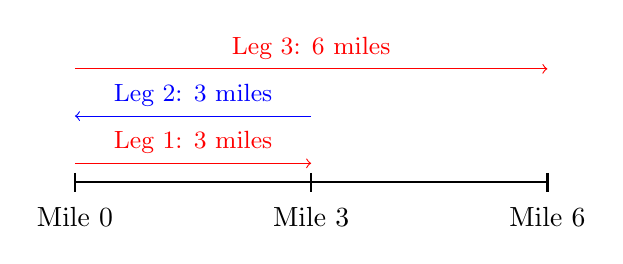
\begin{tikzpicture}
        \draw[thick] (0,0) -- (6,0);

        % major ticks (integers)
        \foreach \x in {0,3, 6}{
            \draw[thick] (\x,0.12) -- (\x,-0.12) node[below,yshift=-2pt] {Mile $\x$};
        }

        \draw[thick] (3, 0.06) -- (3, -0.06);

        \draw[->, red] (0, 0.24) -- (3, 0.24) node[midway, above] {\small Leg 1: 3 miles};
        \draw[->, blue] (3, 0.84) -- (0, 0.84) node[midway, above] {\small Leg 2: 3 miles};
        \draw[->, red] (0, 1.44) -- (6, 1.44) node[midway, above] {\small Leg 3: 6 miles};
    \end{tikzpicture}
\end{center}

Therefore, the total mileage that you've covered is 12 miles. These two questions are the root behind the concepts of $\textbf{displacement}$ and $\textbf{distance}$. \par

\begin{tcolorbox}[definition]
    \begin{tabbing}
        \textit{Displacement} $\rightarrow$ \= Definition: How far apart the starting position and ending position \\ 
        \> are. Note that this value can be positive or negative.
    \end{tabbing} \vspace{11pt}
    \begin{tabbing}
        \textit{Total Distance} $\rightarrow$ \= Definition: How far you travel in total. This value can only be \\ 
        \> positive.
    \end{tabbing} 
\end{tcolorbox}

\begin{center}
    \fbox{\fbox{\begin{minipage}{0.96\textwidth}
        \vspace{11pt}
        Given $v$ is the velocity function and $x$ is the position function, \par
        \vspace{11pt}
        $\hfill \text{Displacement} \rightarrow \int_a^b v \, dt \hfill \text{Total Distance} \rightarrow \int_a^b |v| \, dt \hfill$ \par
        \vspace{11pt}
        $\hfill \text{Position at } t = a \rightarrow x(a) + \int_a^b v \, dt \hfill$
        \vspace{11pt}
    \end{minipage}}}
\end{center}

\begin{tcolorbox}[example]
    \textbf{Ex 3.3.4: } A particle moves along a line so that its velocity at any time $t$ is $v(t) = t^2 + t - 6$ (measured in meters per second). \\
    \begin{enumerate}[label=\hspace{11pt}(\alph*), align=left, leftmargin=*, labelsep=0.25em]
        \item Find the displacement of the particle during the time period $1 \leq t \leq 4$. \\
        \item Find the distance traveled during the time period $1 \leq t \leq 4$. \\
    \end{enumerate}
\end{tcolorbox}
\begin{tcolorbox}[solution]
    \textbf{Sol 3.3.4: } \par
    a) \begin{align*}
        \int_a^b v \, dt & = \int_1^4 \left(t^2 + t - 6\right) \, dt \\[11pt]
        & = \left[\dfrac{t^3}{3} + \dfrac{t^2}{2} - 6t\right]_1^4 \\[11pt]
        & = \boxed{-\dfrac{21}{2} \si{meters}}
    \end{align*}
    b) $v(t) = 0$ when $t = 2$. \begin{align*}
        \int_a^b |v| \, dt & = -\int_1^2 \left(t^2 + t - 6\right) \, dt + \int_2^4 \left(t^2 + t - 6\right) \, dt \\[11pt]
        & = -\left[\dfrac{t^3}{3} + \dfrac{t^2}{2} - 6t\right]_1^2 + \left[\dfrac{t^3}{3} + \dfrac{t^2}{2} - 6t\right]_2^4 \\[11pt]
        & = \boxed{\dfrac{89}{6} \si{meters}}
    \end{align*}
    Make sure to remember your units in your answer! The AP exam will dock points for unitless answers.
\end{tcolorbox}

\newpage

\textbf{\large{3.3 Free Response Homework}} \par

Find the area between the curve of the given equation and the $x$-axis on the given interval. \par

\twoquestion{1a. $y = x^3$ on $x \in [0, \, 2]$}{1b. $y = x^3$ on $x in [-1, \, 2]$} \\[11pt]
\twoquestion{2a. $y = 4x - x^3$ on $x \in [0, \, 2]$}{2b. $y = 4x - x^3$ on $x \in [-1, \, 2]$} \\[11pt]
\twoquestion{3a. $y = \sin (x)$ on $x \in [0, \, \pi]$}{3b. $y = \sin (x)$ on $x \in [-\pi, \, \pi]$} \\[11pt]
\twoquestion{4a. $y = 2x^2 - x^3$ on $x \in [0, \, 2]$}{4b. $2x^2 - x^3$ on $x \in [-1, \, 2]$} \\[11pt]
\twoquestion{5. $y = x^3 - 2x^2 - 3x$ on $x = [-2, \, 2]$}{6. $y = x^3 - 4x^2 + 4x$ on $x \in [-1, 2]$} \\[11pt]
\twoquestion{7. $y = x^3 - 2x^2 - x + 2$ on $x \in [-3, \, 3]$}{8. $y = \dfrac{\pi}{2}\cos (x)\sin (\pi + \pi\sin (x))$ on $x \in \left[-\dfrac{\pi}{2}, \, \pi\right]$} \\[11pt]
\twoquestion{9. $y = -\dfrac{x}{x^2 + 4}$ on $x \in [-2, \, 2]$}{10. $y = \dfrac{4 - x^2}{x^2 + 4}$ on $x \in [-3, \, 3]$} \\[11pt]
\twoquestion{11. $y = \dfrac{\sin \left(\sqrt{x}\right)}{\sqrt{x}}$ on $x \in [0.01, \, \pi^2]$}{12. $y = x\sqrt{18 - 2x^2}$ on $x \in [-2, \, 1]$} \\[11pt]
\twoquestion{13. $y = 3\sin (x)\sqrt{1 - \cos (x)}$ on $x \in \left[-\dfrac{\pi}{2}, \, \dfrac{\pi}{3}\right]$}{14. $y = x^2e^{x^3}$ on $x \in [0, \, 1.5]$} \\[11pt]

Answer the following questions regarding distance and displacement. \par

\onequestion{15. The velocity function (in meters per second) for a particle moving along a line is $v(t) = 3t - 5$.}
\begin{enumerate}[label=\hspace{11pt}(\alph*), align=left, leftmargin=*, labelsep=0.25em]
    \item Find the displacement of the particle during the time period $0 \leq t \leq 3$. 
    \item Find the distance traveled during the time period $0 \leq t \leq 3$. 
\end{enumerate} \vspace{11pt}

\onequestion{16. The velocity function (in meters per second) for a particle moving along a line is $v(t) = t^2 - 2t - 8$.}
\begin{enumerate}[label=\hspace{11pt}(\alph*), align=left, leftmargin=*, labelsep=0.25em]
    \item Find the displacement of the particle during the time period $1 \leq t \leq 6$. 
    \item Find the distance traveled during the time period $1 \leq t \leq 6$. 
\end{enumerate} \vspace{11pt}

For problems \#17-20, show the setup to determine the area and solve the integral. Do not use the absolute value method. \par

\onequestion{17. Find the area under the curve $f(x) = e^{-x^2} - x$ on $x \in [-1, \, 2]$.} \\[11pt]
\onequestion{18. Find the area under the curve $f(x) = e^{-x^2} - 2x$ on $x \in [-1, \, 2]$.} \\[11pt]
\onequestion{19. Find the area under the curve $f(x) = \dfrac{x}{x^2 + 1} + \cos (x)$ on $x \in [0, \, \pi]$.} \\[11pt]
\onequestion{20. Find the area under the curve $g(x) = -1 - x\sin (x)$ on $x \in [0, \, 2\pi]$.} \\[11pt]

\textbf{\large{3.3 Multiple Choice Homework}} \par

\begin{questions}
    \question The graph of $y = f(x)$ is shown below. $A$ and $B$ are positive numbers that represent the areas between the curve and the $x$-axis.
    \begin{center}
        \includegraphics[width = 0.6\textwidth]{\graphicsdir Chapter 3 Graphics/3.3-Graphic5.png}
    \end{center}
    In terms of $A$ and $B$, $\int_{-5}^3 f(x) \, dx + \int_{-2}^3 f(x) \, dx = $ \\

    \begin{oneparchoices}
        \choice $A$
        \choice $A - B$
        \choice $2A - B$
        \choice $A + B$
        \choice $A - 2B$
    \end{oneparchoices} \par \horizontalline

    \question The graph of $y = f(x)$ is shown below. $A$ and $B$ are positive numbers that represent the areas between the curve and the $x$-axis.
    \begin{center}
        \includegraphics[width = 0.6\textwidth]{\graphicsdir Chapter 3 Graphics/3.3-Graphic5.png}
    \end{center}
    In terms of $A$ and $B$, $2\int_{-5}^3 f(x) \, dx + 3\int_{-2}^3 f(x) \, dx = $ \\

    \begin{oneparchoices}
        \choice $A$
        \choice $A - B$
        \choice $2A - B$
        \choice $A + B$
        \choice $A - 2B$
    \end{oneparchoices} \par \horizontalline

    \question The graph of $f(x)$ on $0 \leq x \leq 4$ is shown. 
    \begin{center}
        \includegraphics[width = 0.55\textwidth]{\graphicsdir Chapter 3 Graphics/3.3-Graphic6.png}
    \end{center} \vspace{11pt}
    
    \begin{oneparchoices}
        \choice $-1$
        \choice $0$
        \choice $2$
        \choice $6$
        \choice $12$
    \end{oneparchoices} \par \horizontalline

    \question A particle moves along the $x$-axis so that at any time $t \geq 0$ its velocity is given by $v(t) = \ln (t + 1) - 2t + 1$. What is the total \textbf{distance}, in meters, traveled by the particle during the time interval $0 \leq t \leq 3$? \\

    \begin{oneparchoices}
        \choice $-3.455$
        \choice $0.704$
        \choice $1.540$
        \choice $2.667$
        \choice $4.291$
    \end{oneparchoices} \par \horizontalline

    \question A particle travels along a straight line with a velocity of $v(t) = 3e^{-t^2}\sin (2t)$ meters per second. What is the total \textbf{distance}, in meters, traveled by the particle during the time interval $0 \leq t \leq 2$?

    \begin{oneparchoices}
        \choice $0.835$
        \choice $1.625$
        \choice $1.661$
        \choice $2.261$
        \choice $5.350$
    \end{oneparchoices} \par \horizontalline 

    \question A particle moves along the $x$-axis so that at any time $t \geq 0$ its velocity is given by $v(t) = \ln (t + 1) - 2t + 1$. What is the total \textbf{displacement}, in meters, of the particle during the time interval $0 \leq t \leq 3$ seconds?  \\

    \begin{oneparchoices}
        \choice $-3.455$
        \choice $0.704$
        \choice $1.540$
        \choice $2.667$
        \choice $4.291$
    \end{oneparchoices} \par \horizontalline

    \question A particle travels along a straight line with a velocity of $v(t) = 3e^{-t^2}\sin (2t)$ meters per second. What is the total \textbf{distance}, in meters, traveled by the particle during the time interval $0 \leq t \leq 2$?

    \begin{oneparchoices}
        \choice $0.835$
        \choice $1.625$
        \choice $1.661$
        \choice $2.261$
        \choice $5.350$
    \end{oneparchoices} \par \horizontalline 
\end{questions}